\documentclass[12pt,twoside]{article}

\newcommand{\reporttitle}{Mathematics for Machine Learning}
\newcommand{\reportauthor}{Alexander Gaskell}
\newcommand{\reporttype}{Coursework 2}
\newcommand{\cid}{01813313}

% include files that load packages and define macros
%%%%%%%%%%%%%%%%%%%%%%%%%%%%%%%%%%%%%%%%%
% University Assignment Title Page 
% LaTeX Template
% Version 1.0 (27/12/12)
%
% This template has been downloaded from:
% http://www.LaTeXTemplates.com
%
% Original author:
% WikiBooks (http://en.wikibooks.org/wiki/LaTeX/Title_Creation)
%
% License:
% CC BY-NC-SA 3.0 (http://creativecommons.org/licenses/by-nc-sa/3.0/)
% 
% Instructions for using this template:
% This title page is capable of being compiled as is. This is not useful for 
% including it in another document. To do this, you have two options: 
%
% 1) Copy/paste everything between \begin{document} and \end{document} 
% starting at \begin{titlepage} and paste this into another LaTeX file where you 
% want your title page.
% OR
% 2) Remove everything outside the \begin{titlepage} and \end{titlepage} and 
% move this file to the same directory as the LaTeX file you wish to add it to. 
% Then add \input{./title_page_1.tex} to your LaTeX file where you want your
% title page.
%
%----------------------------------------------------------------------------------------
%	PACKAGES AND OTHER DOCUMENT CONFIGURATIONS
%----------------------------------------------------------------------------------------
\usepackage{ifxetex}
\usepackage{textpos}
\usepackage{natbib}
\usepackage{kpfonts}
\usepackage[a4paper,hmargin=2.8cm,vmargin=2.0cm,includeheadfoot]{geometry}
\usepackage{ifxetex}
\usepackage{stackengine}
\usepackage{tabularx,longtable,multirow,subfigure,caption}%hangcaption
\usepackage{fncylab} %formatting of labels
\usepackage{fancyhdr}
\usepackage{color}
\usepackage[tight,ugly]{units}
\usepackage{url}
\usepackage{float}
\usepackage[english]{babel}
\usepackage{amsmath}
\usepackage{graphicx}
\usepackage[colorinlistoftodos]{todonotes}
\usepackage{dsfont}
\usepackage{epstopdf} % automatically replace .eps with .pdf in graphics
\usepackage{natbib}
\usepackage{backref}
\usepackage{array}
\usepackage{latexsym}
\usepackage{etoolbox}

\usepackage{enumerate} % for numbering with [a)] format 



\ifxetex
\usepackage{fontspec}
\setmainfont[Scale=.8]{OpenDyslexic-Regular}
\else
\usepackage[pdftex,pagebackref,hypertexnames=false,colorlinks]{hyperref} % provide links in pdf
\hypersetup{pdftitle={},
  pdfsubject={}, 
  pdfauthor={\reportauthor},
  pdfkeywords={}, 
  pdfstartview=FitH,
  pdfpagemode={UseOutlines},% None, FullScreen, UseOutlines
  bookmarksnumbered=true, bookmarksopen=true, colorlinks,
    citecolor=black,%
    filecolor=black,%
    linkcolor=black,%
    urlcolor=black}
\usepackage[all]{hypcap}
\fi

\usepackage{tcolorbox}

% various theorems
\usepackage{ntheorem}
\theoremstyle{break}
\newtheorem{lemma}{Lemma}
\newtheorem{theorem}{Theorem}
\newtheorem{remark}{Remark}
\newtheorem{definition}{Definition}
\newtheorem{proof}{Proof}

% example-environment
\newenvironment{example}[1][]
{ 
\vspace{4mm}
\noindent\makebox[\linewidth]{\rule{\hsize}{1.5pt}}
\textbf{Example #1}\\
}
{ 
\noindent\newline\makebox[\linewidth]{\rule{\hsize}{1.0pt}}
}



%\renewcommand{\rmdefault}{pplx} % Palatino
% \renewcommand{\rmdefault}{put} % Utopia

\ifxetex
\else
\renewcommand*{\rmdefault}{bch} % Charter
\renewcommand*{\ttdefault}{cmtt} % Computer Modern Typewriter
%\renewcommand*{\rmdefault}{phv} % Helvetica
%\renewcommand*{\rmdefault}{iwona} % Avant Garde
\fi

\setlength{\parindent}{0em}  % indentation of paragraph

\setlength{\headheight}{14.5pt}
\pagestyle{fancy}
\fancyfoot[ER,OL]{\thepage}%Page no. in the left on
                                %odd pages and on right on even pages
\fancyfoot[OC,EC]{\sffamily }
\renewcommand{\headrulewidth}{0.1pt}
\renewcommand{\footrulewidth}{0.1pt}
\captionsetup{margin=10pt,font=small,labelfont=bf}


%--- chapter heading

\def\@makechapterhead#1{%
  \vspace*{10\p@}%
  {\parindent \z@ \raggedright %\sffamily
        %{\Large \MakeUppercase{\@chapapp} \space \thechapter}
        %\\
        %\hrulefill
        %\par\nobreak
        %\vskip 10\p@
    \interlinepenalty\@M
    \Huge \bfseries 
    \thechapter \space\space #1\par\nobreak
    \vskip 30\p@
  }}

%---chapter heading for \chapter*  
\def\@makeschapterhead#1{%
  \vspace*{10\p@}%
  {\parindent \z@ \raggedright
    \sffamily
    \interlinepenalty\@M
    \Huge \bfseries  
    #1\par\nobreak
    \vskip 30\p@
  }}
  



% %%%%%%%%%%%%% boxit
\def\Beginboxit
   {\par
    \vbox\bgroup
	   \hrule
	   \hbox\bgroup
		  \vrule \kern1.2pt %
		  \vbox\bgroup\kern1.2pt
   }

\def\Endboxit{%
			      \kern1.2pt
		       \egroup
		  \kern1.2pt\vrule
		\egroup
	   \hrule
	 \egroup
   }	

\newenvironment{boxit}{\Beginboxit}{\Endboxit}
\newenvironment{boxit*}{\Beginboxit\hbox to\hsize{}}{\Endboxit}



\allowdisplaybreaks

\makeatletter
\newcounter{elimination@steps}
\newcolumntype{R}[1]{>{\raggedleft\arraybackslash$}p{#1}<{$}}
\def\elimination@num@rights{}
\def\elimination@num@variables{}
\def\elimination@col@width{}
\newenvironment{elimination}[4][0]
{
    \setcounter{elimination@steps}{0}
    \def\elimination@num@rights{#1}
    \def\elimination@num@variables{#2}
    \def\elimination@col@width{#3}
    \renewcommand{\arraystretch}{#4}
    \start@align\@ne\st@rredtrue\m@ne
}
{
    \endalign
    \ignorespacesafterend
}
\newcommand{\eliminationstep}[2]
{
    \ifnum\value{elimination@steps}>0\leadsto\quad\fi
    \left[
        \ifnum\elimination@num@rights>0
            \begin{array}
            {@{}*{\elimination@num@variables}{R{\elimination@col@width}}
            |@{}*{\elimination@num@rights}{R{\elimination@col@width}}}
        \else
            \begin{array}
            {@{}*{\elimination@num@variables}{R{\elimination@col@width}}}
        \fi
            #1
        \end{array}
    \right]
    & 
    \begin{array}{l}
        #2
    \end{array}
    &%                                    moved second & here
    \addtocounter{elimination@steps}{1}
}
\makeatother

%% Fast macro for column vectors
\makeatletter  
\def\colvec#1{\expandafter\colvec@i#1,,,,,,,,,\@nil}
\def\colvec@i#1,#2,#3,#4,#5,#6,#7,#8,#9\@nil{% 
  \ifx$#2$ \begin{bmatrix}#1\end{bmatrix} \else
    \ifx$#3$ \begin{bmatrix}#1\\#2\end{bmatrix} \else
      \ifx$#4$ \begin{bmatrix}#1\\#2\\#3\end{bmatrix}\else
        \ifx$#5$ \begin{bmatrix}#1\\#2\\#3\\#4\end{bmatrix}\else
          \ifx$#6$ \begin{bmatrix}#1\\#2\\#3\\#4\\#5\end{bmatrix}\else
            \ifx$#7$ \begin{bmatrix}#1\\#2\\#3\\#4\\#5\\#6\end{bmatrix}\else
              \ifx$#8$ \begin{bmatrix}#1\\#2\\#3\\#4\\#5\\#6\\#7\end{bmatrix}\else
                 \PackageError{Column Vector}{The vector you tried to write is too big, use bmatrix instead}{Try using the bmatrix environment}
              \fi
            \fi
          \fi
        \fi
      \fi
    \fi
  \fi 
}  
\makeatother

\robustify{\colvec}

%%% Local Variables: 
%%% mode: latex
%%% TeX-master: "notes"
%%% End: 
 % various packages needed for maths etc.
% quick way of adding a figure
\newcommand{\fig}[3]{
 \begin{center}
 \scalebox{#3}{\includegraphics[#2]{#1}}
 \end{center}
}

%\newcommand*{\point}[1]{\vec{\mkern0mu#1}}
\newcommand{\ci}[0]{\perp\!\!\!\!\!\perp} % conditional independence
\newcommand{\point}[1]{{#1}} % points 
\renewcommand{\vec}[1]{{\boldsymbol{{#1}}}} % vector
\newcommand{\mat}[1]{{\boldsymbol{{#1}}}} % matrix
\newcommand{\R}[0]{\mathds{R}} % real numbers
\newcommand{\Z}[0]{\mathds{Z}} % integers
\newcommand{\N}[0]{\mathds{N}} % natural numbers
\newcommand{\nat}[0]{\mathds{N}} % natural numbers
\newcommand{\Q}[0]{\mathds{Q}} % rational numbers
\ifxetex
\newcommand{\C}[0]{\mathds{C}} % complex numbers
\else
\newcommand{\C}[0]{\mathds{C}} % complex numbers
\fi
\newcommand{\tr}[0]{\text{tr}} % trace
\renewcommand{\d}[0]{\mathrm{d}} % total derivative
\newcommand{\inv}{^{-1}} % inverse
\newcommand{\id}{\mathrm{id}} % identity mapping
\renewcommand{\dim}{\mathrm{dim}} % dimension
\newcommand{\rank}[0]{\mathrm{rk}} % rank
\newcommand{\determ}[1]{\mathrm{det}(#1)} % determinant
\newcommand{\scp}[2]{\langle #1 , #2 \rangle}
\newcommand{\kernel}[0]{\mathrm{ker}} % kernel/nullspace
\newcommand{\img}[0]{\mathrm{Im}} % image
\newcommand{\idx}[1]{{(#1)}}
\DeclareMathOperator*{\diag}{diag}
\newcommand{\E}{\mathds{E}} % expectation
\newcommand{\var}{\mathds{V}} % variance
\newcommand{\gauss}[2]{\mathcal{N}\big(#1,\,#2\big)} % gaussian distribution N(.,.)
\newcommand{\gaussx}[3]{\mathcal{N}\big(#1\,|\,#2,\,#3\big)} % gaussian distribution N(.|.,.)
\newcommand{\gaussBig}[2]{\mathcal{N}\left(#1,\,#2\right)} % see above, but with brackets that adjust to the height of the arguments
\newcommand{\gaussxBig}[3]{\mathcal{N}\left(#1\,|\,#2,\,#3\right)} % see above, but with brackets that adjust to the height of the arguments
\DeclareMathOperator{\cov}{Cov} % covariance (matrix) 
\ifxetex
\renewcommand{\T}[0]{^\top} % transpose
\else
\newcommand{\T}[0]{^\top}
\fi
% matrix determinant
\newcommand{\matdet}[1]{
\left|
\begin{matrix}
#1
\end{matrix}
\right|
}



%%% various color definitions
\definecolor{darkgreen}{rgb}{0,0.6,0}

\newcommand{\blue}[1]{{\color{blue}#1}}
\newcommand{\red}[1]{{\color{red}#1}}
\newcommand{\green}[1]{{\color{darkgreen}#1}}
\newcommand{\orange}[1]{{\color{orange}#1}}
\newcommand{\magenta}[1]{{\color{magenta}#1}}
\newcommand{\cyan}[1]{{\color{cyan}#1}}


% redefine emph
\renewcommand{\emph}[1]{\blue{\bf{#1}}}

% place a colored box around a character
\gdef\colchar#1#2{%
  \tikz[baseline]{%
  \node[anchor=base,inner sep=2pt,outer sep=0pt,fill = #2!20] {#1};
    }%
}%
 % short-hand notation and macros

\renewcommand{\thesubsection}{\thesection.\alph{subsection}}

%%%%%%%%%%%%%%%%%%%%%%%%%%%%

\begin{document}
% front page
% Last modification: 2016-09-29 (Marc Deisenroth)
\begin{titlepage}

\newcommand{\HRule}{\rule{\linewidth}{0.5mm}} % Defines a new command for the horizontal lines, change thickness here


%----------------------------------------------------------------------------------------
%	LOGO SECTION
%----------------------------------------------------------------------------------------


\includegraphics[width = 4cm]{./figures/imperial}\\[0.5cm] 

\begin{center} % Center remainder of the page

%----------------------------------------------------------------------------------------
%	HEADING SECTIONS
%----------------------------------------------------------------------------------------
\textsc{\LARGE \reporttype}\\[1.5cm] 
\textsc{\Large Imperial College London}\\[0.5cm] 
\textsc{\large Department of Computing}\\[0.5cm] 
%----------------------------------------------------------------------------------------
%	TITLE SECTION
%----------------------------------------------------------------------------------------

\HRule \\[0.4cm]
{ \huge \bfseries \reporttitle}\\ % Title of your document
\HRule \\[1.5cm]
\end{center}
%----------------------------------------------------------------------------------------
%	AUTHOR SECTION
%----------------------------------------------------------------------------------------

%\begin{minipage}{0.4\hsize}
\begin{flushleft} \large
\textit{Author:}\\
\reportauthor~(CID: \cid) \\% Your name 
\textit{Email:} \\
\reportemail
\end{flushleft}
\vspace{2cm}
\makeatletter
Date: \@date 

\vfill % Fill the rest of the page with whitespace



\makeatother


\end{titlepage}




%%%%%%%%%%%%%%%%%%%%%%%%%%%% Main document
\section{Differentiation}
\subsection[]{}
\textbf{[3 marks] Write $f_1(x)$ in the completed square form $\mathbf{(x-c)^T C(x-c) + c_0}$, i.e., determine $\mathbf{C, c, c_0}$.}

\begin{align}
    f_1(x) 
    & = \mathbf{x^TBx - x^Tx + a^Tx - b^Tx} \label{f1} \\
    & = \mathbf{x^T(B-I_2)x + a^Tx - b^Tx} \label{f1_1}
\end{align}
Objective: write equation \ref{f1_1} in completed square form. We can expand the completed square form:
\begin{align}
    \mathbf{(x-c)^T C(x-c) + c_0} 
    & = \mathbf{x^TCx - c^TCx - x^TCc + c^TCc + c_0}
    \label{sq_1}
\end{align}
Equating coefficients on $\mathbf{x^Tx}$ term gives:
\begin{align}
    \mathbf{C = B-I_2} \label{C}
    = \begin{bmatrix} 3 & -2 \\ -2 & 3 \end{bmatrix}
\end{align}
We can exploit the symmetry of $\mathbf{C}$ to write equation \ref{sq_1} as:  
\begin{align}
    \mathbf{(x-c)^T C(x-c) + c_0} 
    & = \mathbf{x^TCx - 2c^TCx + c^TCc + c_0} \label{f1_2}
\end{align}
Comparing coefficients on $\mathbf{x}$ terms in equations \ref{f1_1} and \ref{f1_2} we can see that: 
\begin{align}
    \mathbf{-2c^TC = a^T - b^T} \label{cT_1}
\end{align}
Solve for $\mathbf{c}$:
\begin{align}
    \mathbf{c} 
    & = -\frac{1}{2}\mathbf{C^{-1}(a-b)} \\
    & = -\frac{1}{2}\begin{pmatrix}\frac{1}{5}\begin{bmatrix} 3 & 2 \\ 2 & 3 \end{bmatrix} \end{pmatrix} \colvec{2,0} \\
    & = \colvec{-3/5, -2/5}
\end{align}
Comparing equations \ref{f1_1} and \ref{f1_2} we can solve for $c_0$:
\begin{align}
    \mathbf{c_0} & = -\mathbf{c^TCc} \\ & = -3/5
\end{align}
Hence:
\begin{align}
    \mathbf{C} = \begin{bmatrix} 3 & -2 \\ -2 & 3 \end{bmatrix} \quad , \quad \mathbf{c} = \colvec{-3/5, -2/5} \quad , \quad
    \mathbf{c_0} = -3/5
\end{align}

\pagebreak

\subsection[]{}
\label{b}
\textbf{[2 marks] Explain how you can tell that $f_1$ has a minimum point. State the minimum value of $f_1$ and find the input which achieves this minimum.}
\bigbreak
Begin by computing the gradient of $f_1(x)$ by use of the product rule:
\begin{align}
    \frac{df_1}{d\mathbf{x}} 
    & = g^T\frac{\partial h}{\partial \mathbf{x}} + h^T\frac{\partial g}{\partial \mathbf{x}} \quad \text{where} \quad h(\mathbf{x}) = \mathbf{x-c},\quad g(\mathbf{x}) = \mathbf{C(x-c)} \\
    & = \mathbf{(x-c)^TC^T + (x-c)^TC} \\
    & = \mathbf{2(x-c)^TC} \quad \in \mathbb{R}^{1x2}
\end{align}
The final step exploits the symmetry of $\textbf{C}$. If $f_1$ has a minimum, then the Hessian will be positive definite. Hence we need to find the Hessian and check if it is positive definite:
\begin{align}
    \mathbf{H} 
    & = \begin{bmatrix} \frac{\partial^2 f}{\partial \mathbf{x}^2} \end{bmatrix} \\
    & = \frac{\partial}{\partial \mathbf{x}}(\mathbf{2(x-c)^TC}) \\
    & = 2\mathbf{C^T} \quad \in \mathbb{R}^{2x2}
\end{align}
We can compute the Eigenvalues of $\mathbf{H}$ to be 10 and 2. As both are positive, the Hessian is positive definite, so $f_1$ will have a minimum point.
\smallbreak
The minimum is found by setting the gradient to zero:
\begin{align}
    & \frac{df_1}{d\mathbf{x}} 
    = 0 = \mathbf{2(x-c)^TC} \\
    & \iff \mathbf{x = c} = \colvec{-3/5, -2/5}
\end{align}
At the minimum point:
\begin{align}
    f_1(\mathbf{x}) = \mathbf{c_0} = -3/5
\end{align}

\bigbreak
\pagebreak


\subsection{}
\textbf{[6 marks] Write three python functions grad\_f1(x), grad\_f2(x) and grad\_f3(x) that return the gradient for each of the functions above. All functions must accept numpy (2, ) array inputs and return numpy (2, ) outputs.}
\bigbreak

As found in \ref{b}, the gradient of $f_1$ is:
\begin{align}
    \frac{df_1}{d\mathbf{x}} = \mathbf{2(x-c)^TC} \quad \in \mathbb{R}^{1x2}
\end{align}
The gradient of $f_2$ is:
\begin{align}
    \frac{df_2}{d\mathbf{x}} = -\operatorname{sin} \begin{pmatrix}\mathbf{(x-b)^T(x-b)} \end{pmatrix} \begin{pmatrix}2\mathbf{(x-b)^T}\end{pmatrix} + \mathbf{2(x-a)^TB} \quad \in \mathbb{R}^{1x2}
\end{align}
The gradient of $f_3$ is:
\begin{align}
    \frac{df_3}{d\mathbf{x}} 
    & = \operatorname{exp} \begin{pmatrix} \mathbf{(x-a)^T(x-a)} \end{pmatrix} \begin{pmatrix} 2 \mathbf{(x-a)^T}\end{pmatrix} + \operatorname{exp} \begin{pmatrix} \mathbf{(x-b)^TB(x-b)} \end{pmatrix} \begin{pmatrix} 2 \mathbf{(x-b)^TB}\end{pmatrix} \\
    & \quad + \frac{1}{10}\frac{2}{\mathbf{x^Tx} + \frac{1}{100}}\mathbf{x^T} \quad \in \mathbb{R}^{1x2} \nonumber
\end{align}
The gradient for $f_3$ takes $\mathbf{x} = \colvec{x_1,x_2}$ and exploits the fact that the log determinant term of $f_3$ can be written as:
\begin{align}
    \operatorname{log} \operatorname{det} \begin{pmatrix} \frac{1}{100}I_2 + \mathbf{xx^T} \end{pmatrix} 
    & = \operatorname{log} \begin{pmatrix} \begin{bmatrix} x_1^2 + \frac{1}{100} & x_1x_2 \\
    x_2x_1 & x_2^2 + \frac{1}{100} \end{bmatrix} \end{pmatrix}  \\
    & = \operatorname{log} \begin{pmatrix} {(x_1^2 + \frac{1}{100})(x_2^2 + \frac{1}{100}}) - x_1^2x_2^2 \end{pmatrix} \\
    & = \operatorname{log} \begin{pmatrix} \frac{1}{100} ( {x_1^2 + x_2^2 + \frac{1}{100}}) \end{pmatrix} \\
    & = \operatorname{log} \begin{pmatrix} \frac{1}{100} ( {\mathbf{x^Tx} + \frac{1}{100}}) \end{pmatrix}
\end{align}
\pagebreak

\subsection[]{}
\textbf{[4 marks] Use your gradients to implement a gradient descent algorithm with 50 iterations to find a local minimum for both $f_2$ and $f_3$. Show the steps of your algorithm on a contour plot of the function. Start from the point (0.3, 0) and state the step size you used. Produce separate contour plots for the two functions, using first component of x on the x axis and the second on the y.}

\begin{figure}[h]
\centering % this centers the figure
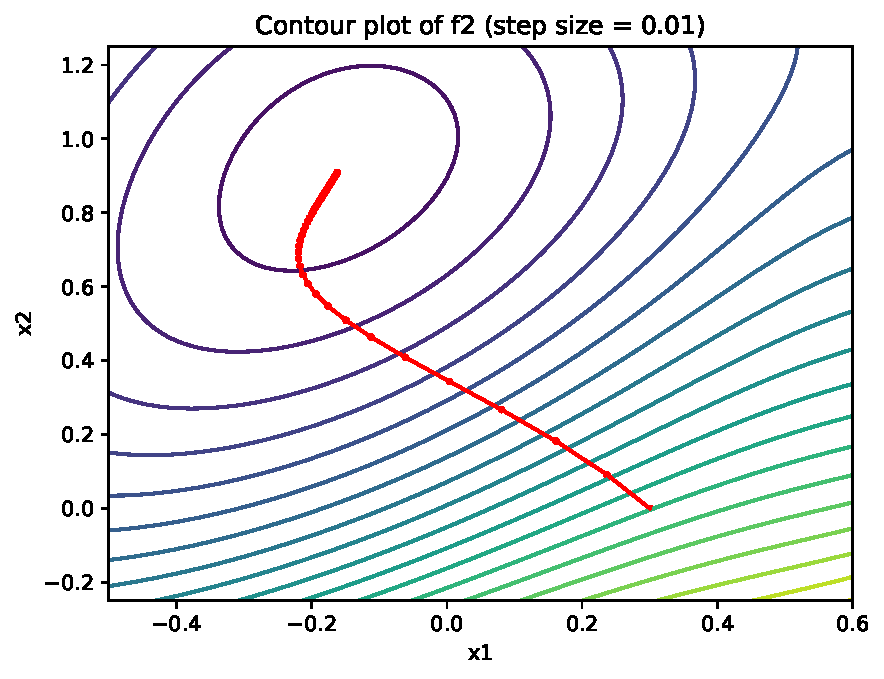
\includegraphics[width = 0.65\hsize]{./figures/contour_f2.pdf} % this includes the figure and %specifies that it should span 0.7 times the horizontal size of the page
\caption{Contour plot for $f_2$ with gradient descent}% caption of the figure
\label{fig:f2}
\end{figure}

\begin{figure}[h]
\centering % this centers the figure
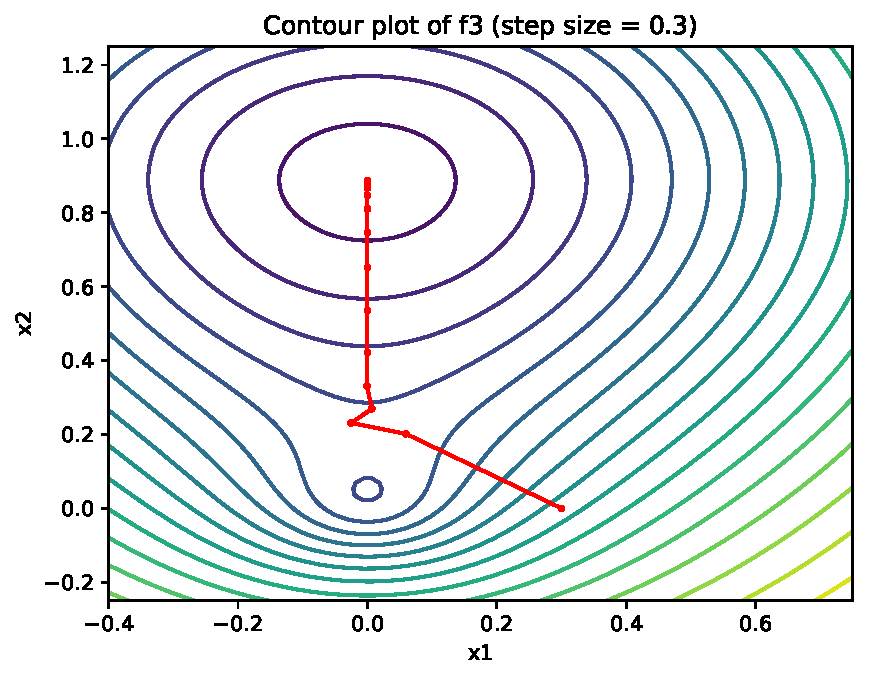
\includegraphics[width = 0.65\hsize]{./figures/contour_f3.pdf} % this includes the figure and %specifies that it should span 0.7 times the horizontal size of the page
\caption{Contour plot for $f_3$ with gradient descent} % caption of the figure
\label{fig:f3}
\end{figure}
\pagebreak



\subsection[]{}
\textbf{[5 marks] For the two functions f2 and f3:
\begin{itemize}
    \item Discuss the qualitative differences you observe when performing gradient descent with step sizes varying between 0.01 and 1, again starting the point (0.3, 0)
    \item \textbf{Briefly describe also what happens in the two cases with grossly mis-specified step-sizes (i.e. greater than 1).}
\end{itemize}}
\bigbreak
Varying the step size between $0.01$ and $1$ illustrates the careful balance that must be struck when choosing the step size for gradient descent: if the learning rate is too small, the function will take a large number of training iterations to converge and amy get stuck at local minima; if the learning rate is too large, gradient descent will overshoot the minimum point, meaning a long time to convergence or even divergence in some cases. 
\\ \\
In figure \ref{fig:f2}, plotted gradient descent using a step size of 0.01 is plotted for $f_2$. This is an appropriate value to choose as we have a sufficient number of training iterations to converge to the (global) minimum. However, a learning rate of 0.01 is inappropriate to use for $f_3$ for two reasons: the step size is too small for convergence of any kind (given 50 training iterations the path does not reach any minimum point). Additionally, $f_3$ gets stuck at a local minimum (located at approx $(0.00, 0.05)$) with any learning rate less than approx 0.25. Hence having a learning rate which is too low can make gradient descent liable to getting stuck at local minima and expensive as more training iterations are required for convergence.
\\ \\
Having a step size which is too large presents other difficulties: gradient descent can overshoot the minimum point meaning more training iterations until convergence, with no convergence/divergence possible in some circumstances. For example, once learning rate is between 0.6 and 1 for $f_3$, then the path of convergence is very jagged and oscillates around the minimum point. Similar behaviour is seen from $f_2$ if we set the step size around 0.1. However, once the learning rate is above 0.175 for $f_2$, gradient descent exhibits divergence (i.e. oscillating around the minimum point but overshooting so dramatically with each step that the minimum gets further away with each iteration). This divergence behaviour becomes even more severe when we increase the step size further.
\\ \\
For $f_2$, if we severely mis-specify the step size (e.g. set = 2), then we see simply a more extreme version of the divergence described above. The point where divergence begins occurring is 0.175, so if the step size is larger than this we will see divergence. For $f_3$, we do not see divergence in the same way as we saw for $f_2$, even if the step-size is inappropriately high. For example, when we set the learning rate to 10, gradient descent massively overshoots the minimum and oscillates around it without properly converging; however, the gradient does not explode in the same way as it does for $f_2$. 




\end{document}
%%% Local Variables: 
%%% mode: latex
%%% TeX-master: t
%%% End: 
